\section{OpenCL}
\label{sec:opencl}

\subsection{What is OpenCL?}
OpenCL is specified by the Khronos Group in the OpenCL 1.2 Specification as follows:

\begin{quote}
OpenCL (Open Computing Language) is an open royalty-free standard for general purpose
parallel programming across CPUs, GPUs and other processors, giving software developers
portable and efficient access to the power of these heterogeneous processing platforms. \cite{opencl_spec}
\end{quote}

The Khronos Group is an industry consortium who maintains OpenCL as an open standard. This means that the Khronos Group offers a specification of the OpenCL API and a detailed description about its functionality and behavior for free. This specification can be downloaded at their website \cite{opencl_spec}. Maintaining the OpenCL standard consequently means, that the Khronos Group neither provides software development kits (SDKs), drivers that implement OpenCL nor hardware that it can make use of. These concerns are subject to other companies called vendors, which are typically hardware manufacturers providing necessary developing resources and include OpenCL support in their drivers. Examples of such companies are the two famous graphic card vendors NVIDIA and AMD as well as the renowned processor manufacturer Intel.

Unlike other famous APIs the Khronos Groups specifies which are very specific in their usage or the targeted hardware (like the famous 3D API OpenGL used to drive graphic hardware), OpenCL is a general purpose programming framework. It was conceived with universality in mind, offering almost no restrictions on the field of application it may be used in. Portability from its well designed hardware abstraction model, which enables it to run on many different kinds of devices, even ones which may have not been created yet, is one of OpenCL most powerful strengths. Such devices may be classical CPUs and GPUs, but also more uncommon types of hardware like FPGAs (field programmable gate arrays), DSPs (digital signal processors) or Intel's MICs (Many Integrated Core) \cite{mic}. Moreover, OpenCL may be used to combine multiple available devices into a single heterogeneous platform extending an applications processing resources beyond the bounds of individual pieces of hardware.

Additionally to being independent of a specific purpose and decoupled from the underlying hardware, OpenCL is also available across all mayor operations systems including Windows, Linux and Mac OS X.

With the upcoming specification of WebCL (currently available as a working draft), OpenCL will eventually even find its way into web browsers and the HTML5 technology. Thus making it even independent of an operating system and bringing high performance computing into web applications.

\subsection{Components}

OpenCL is not an API alone. As it allows programs to run on hardware that may have certain restrictions or offer different features than a classical CPU, traditional languages like C++, Java or C\# can not be used to write those programs. Therefore, the OpenCL standard includes the specification of a separate language that is used to write small programs that are executed on a hardware device. These programs are called kernels and are written in the OpenCL C language, which is a restricted version of C99 with extensions for vectorization and handling OpenCL's abstract memory model.

\pagebreak

To allow OpenCL to support many different hardware platforms it consists of the following components:

\begin{description}
	\item[API] \hfill \\
	The application programming interface is specified by the Khronos Group, ensuring that every vendor implementation of OpenCL is compatible and exchangeable. The API is provided as a set of C header files that a software developer can download from Khronos' website. These headers are typically also shipped within an SDK. Khronos additionally specifies a C++ wrapper around C API. Bindings for other languages exist but they are not maintained by Khronos.
	The API is used by a conventional program (e.g. written in C++) to run kernels on an OpenCL capable device. This program is called the host application.
	\item[SDK] \hfill \\
	The software developing kit is the main collection of tools and resources a software developer needs to write applications using OpenCL. An SDK is usually provided by a vendor, an implementor of OpenCL. Examples of such SDKs are the NVIDIA CUDA Toolkit and AMD's Accelerated Parallel Processing (APP) SDK. These SDKs typically contain header files to be included by a C/C++ program and static libraries for the linker, which are responsible for binding to the OpenCL driver at runtime. Furthermore, code examples, tutorials, documentation, developing tools etc. may be additionally provided depending on the vendor. With headers and static libraries an SDK contains all resources necessary to write and compile an OpenCL application.
	\item[OpenCL C language] \hfill \\
	Kernels are typically written in separate source files using the OpenCL C language. An OpenCL application reads these source files at run time and sends them to the OpenCL compiler to create a binary for one or more available hardware devices where it may be executed. A source file written in the OpenCL C language may consist of several functions, variable definitions, control flow statements, comments, etc., but has to have at least one function prefixed with the \lstinline!__kernel! attribute. This function may be called by the host application through the OpenCL API and serves as an entry point into a kernel.
	\item[OpenCL C Compiler] \hfill \\
	OpenCL kernels must be compiled for a specific platform before they can be executed. This compilation process is initiated and controlled by the host application through the API. The separate compilation at run time is required to retain OpenCL's portability, as an OpenCL application may be deployed on any kind of machine with a suitable driver. Consequently, the available OpenCL implementation (providing the compiler) and the used hardware device (affecting the compiler's output) may only be determined at runtime.
	\item[Driver] \hfill \\
	Finally, the driver is OpenCL's core. It implements the OpenCL API and maps the functionality specified in the standard to a vendor's hardware. The host application uses the driver through the API to initialize OpenCL, compile kernels, allocate memory resources, initiate computations and communicate with kernels running on a device. A driver is always specific to a dedicated hardware and must therefore be provided by a vendor. The driver is sometimes also referred to as Installable Client Driver (ICD).
\end{description}

\subsection{Hardware architectures}
\label{sec:hardware_arch}

One of the greatest advantages of OpenCL and also one of the biggest influences on its design is OpenCL's ability to support devices of many different hardware architectures. These devices can be used through OpenCL by the same common API and may even be used together in a single application or computation, which is sometimes referred to as heterogeneous computing.
A closer look into the architectures of the two most common hardware devices, namely a CPU and a GPU, may aid the reader to better understand design decisions made by the Khronos Group when OpenCL was conceived. Furthermore, a deeper understanding of graphics hardware will be needed for the implementation chapters of this thesis.

\subsubsection{Central Processing Unit (CPU)}

The CPU is the kind of processors developers are mostly used to. Software written in common languages like C++, Java or C\# is directly or indirectly (using a Virtual Machine) executed on this kind of hardware.
In figure \ref{fig:ivy_bridge} we can see the design of a modern processor by the example of an Intel Ivy Bridge quad-core. One can clearly see the four physical cores of the processor. Thanks to hardware multithreading (Hyper-threading in Intel terms) each physical core can process a pair of threads which are seen as two virtual CPUs by the operation system resulting in 8 available cores for an application.
Note the on-chip graphics processor in the Ivy Bridge architecture which can be used as a replacement for a graphics card. It is however not used as general processing device such as the CPU's cores.

\begin{figure}
\centering
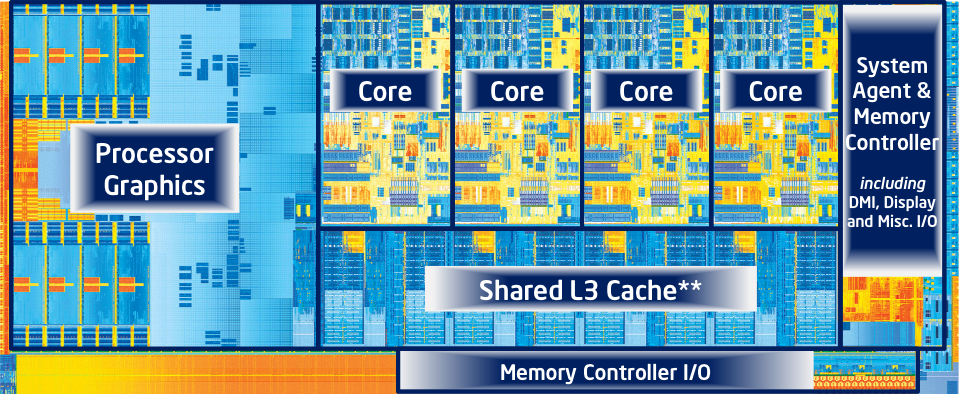
\includegraphics[width=0.9\textwidth]{ivy_bridge}
\caption{Architectural overview of an Intel Ivy Bridge processor. \cite{ivy_bridge}}
\label{fig:ivy_bridge}
\end{figure}

When it comes down to calculative throughput, and the tackled problem offers some degree of data parallelism (several chunks of data are processed equally), SIMD (Single Instruction Multiple Data) features of the CPU can be used to increase the number of input elements an instruction can process. Intel's Ivy Bridge for example allows the parallel execution (vectorization) of up eight single precision floating point operations using AVX (Advanced Vector Extensions, successor of SSE - Streaming SIMD Extensions) instructions.

Considering memory access, the CPU uses the standard data bus to communicate with the external main memory. As this communication usually takes a while (up to hundreds or even thousands of CPU cycles \cite[p.54]{opencl_book}), the CPU uses a hierarchical cache system. Each core has it's own level one and level two cache, which have to be kept synchronized to the other cores. All cores share a common level three cache that is further connected to the memory controller.

From a performance concerned developer's perspective, all we have to pay attention to is to have enough parallelism in our application to utilize all cores of our CPU (which is typically a number of 2, 4 or 8 on consumer hardware). If our application has to process large amounts of data using the same operations on elements of the input (e.g. multimedia applications like image or video processing), vector instructions may be used to speed up execution. Regarding memory, beside small adjustments to improve cache effects the developer has only limited power to optimize, as the entire cache system is controlled by the CPU and operation system. 


\subsubsection{Graphics Processing Unit (GPU)}
\label{sec:gpu}

When we think of a GPU we think of a highly parallel, graphics orientated processing device. From its introduction with OpenGL in 1989 until the creation of the first GPGPU languages in 2004 (cf. chapter \ref{sec:history}), the architecture of a GPU's hardware followed the principles of the graphics pipeline. To fit this purpose, GPUs developed from original desktop processors to (as written in the book Heterogeneous Computing with OpenCL \cite{opencl_book}) heavily multithreaded devices employing sophisticated task management directly in hardware. This was needed to cope with complex task graphs processing vertices, geometry and pixels. This tasks and the data they process are highly parallel and represent an extensive amount of independent work, which is therefore most suitably handled by a device with a great amount of cores employing latency tolerant multithreading\footnote{Latency tolerant processing units are characterized by being insensitive to longer lasting memory requests.}.

\begin{figure}
\centering
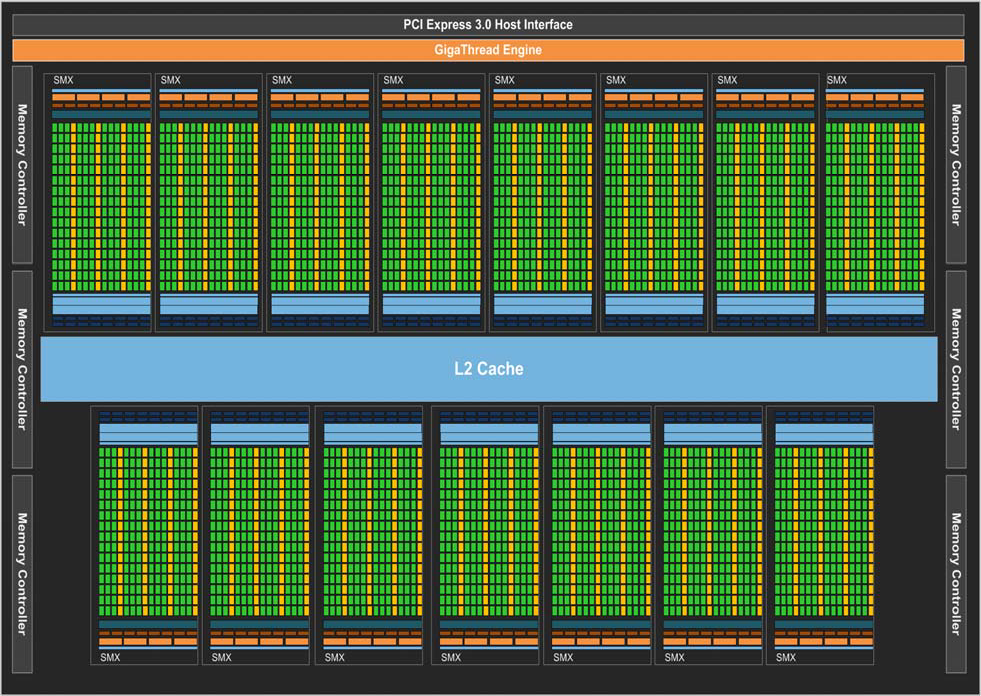
\includegraphics[width=0.9\textwidth]{kepler_arch}
\caption{Full chip block diagram of NVIDIA's Kepler GK110 architecture containing 15 streaming multiprocessors (SMX). \cite{kepler_arch}}
\label{fig:kepler_arch}
\end{figure}

\begin{figure}
\centering
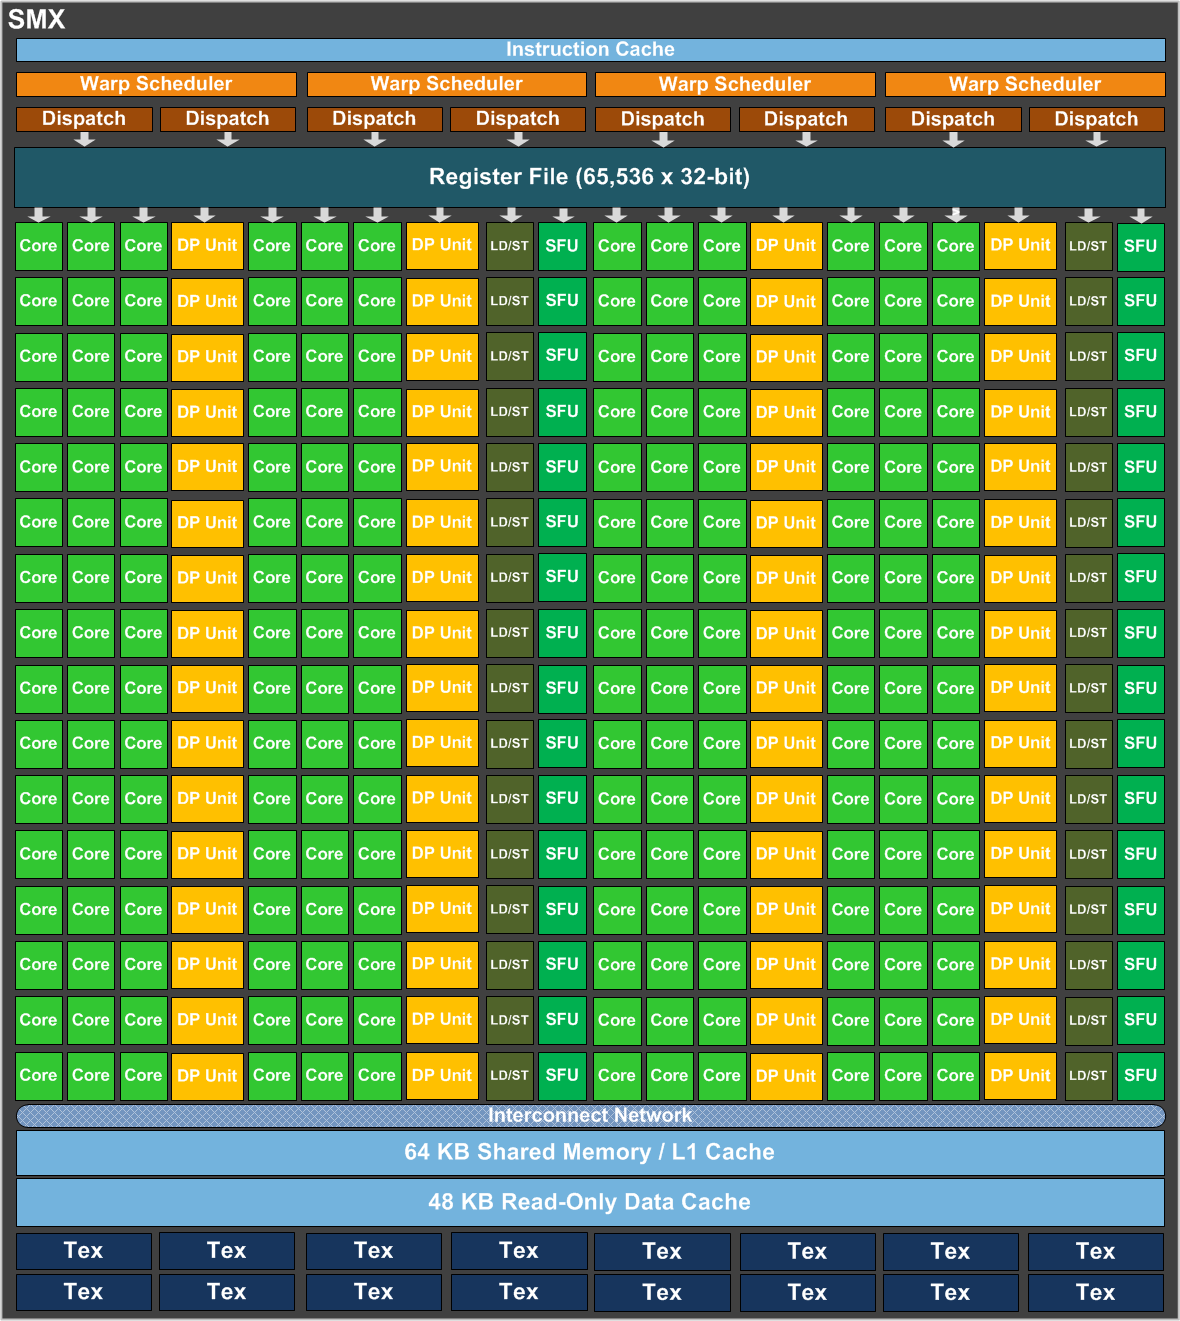
\includegraphics[width=0.9\textwidth]{kepler_arch_smx}
\caption{Architecture of a Streaming Multiprocessor (SMX) of NVIDIA's Kepler GK110 architecture containing 192 single precision CUDA cores, 64 double precision units, 32 special function units (SFU), and 32 load/store units (LD/ST) \cite{kepler_arch}.}
\label{fig:kepler_arch_smx}
\end{figure}

In figure \ref{fig:kepler_arch} we can see the design of a modern GPU by the example of NVIDIA's Kepler architecture. On the top side of the block diagram the PCI Express controller is placed. This interface is responsible for the communication of the graphics card with the CPU through the mainboard's PCI Express bus. After data has arrived at the graphics device, it has to be scheduled for processing to one or more of the streaming multiprocessors (SM, or SMX in NVIDIA's Kepler architecture terms). A SM is an aggregation of many cores with additional scheduling logic and therefore representing an extra hierarchical step in a GPU's workflow. This is one of the first bigger differences in the architecture of modern GPUs when compared with traditional CPUs. SMs are called compute units in OpenCL terms.

Figure \ref{fig:kepler_arch_smx} shows a detailed view of the structure of a streaming multiprocessors. Once a package of work is scheduled to a SM, it is then prepared for execution by the Warp Schedulers. A Warp is a block of threads (32 on NVIDIA hardware) executing the same instructions in parallel along cores managed by the Warp Scheduler. This concept is sometimes called SIMT (Single Instruction Multiple Threads). The difference to SIMD (Single Instruction Multiple Data) is that SIMD requires a vector instruction in each thread whereas SIMT only uses scalar code; the vectorization is handled by the hardware \cite[p.99]{gpu_optimizations}. A Warp Scheduler is able to manage multiple Warps at the same time (up to 64 on the Kepler GK110 architecture \cite[p.7]{kepler_arch}), which may be executed interleaved on the cores (similar to the two threads on a hyper-threading Intel core). This allows to hide memory latency (latency tolerance), because when a Warp has to stall because of a memory request, the Warp Scheduler can execute other Warps until the memory request is satisfied.

%\begin{figure}
%\centering
%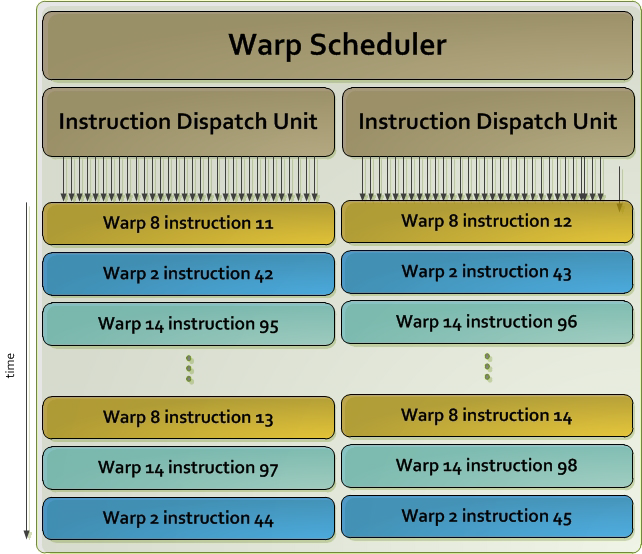
\includegraphics[width=0.5\linewidth]{warp_scheduler}
%\caption{Closer look on a Warp Scheduler. Each Warp Scheduler has two dispatcher units %allowing the execution of two independent instructions of a Warp in parallel. %\cite{kepler_arch}}
%\label{fig:warp_scheduler}
%\end{figure}

Another important thing to notice is that all cores within a SM share the same registers. This plays an important role when choosing the right number of Warps to run concurrently on the SM. Too less Warps may result in unused core cycles whereas a too large number of Warps may request more registers than there are available at the SM. The additionally needed registers are then allocated in the slow global memory. This concern will be discussed later in chapter \ref{sec:execution_model}.

The actual work is then performed on the cores itself. The major number of cores (labeled "Core" in green in figure \ref{fig:kepler_arch_smx}) are used for single precision floating point and integer arithmetics. In contrast to older GPUs, modern graphics processing units also include support for double precision floating point arithmetic, which was not needed for graphical calculations in the past, but becomes increasingly important in GPGPU computing. The Kepler architecture serves this need by dedicated cores (labeled "DP Unit"). Additional hardware resources include the load and store unit for register and memory access and the special function unit (labeled "SFU"). On the bottom of figure \ref{fig:kepler_arch_smx} we find the texture units which are heavily used in 3D graphics. They can also be used by OpenCL via images (more in chapter \ref{sec:images}).

Finally, beside the way of executing threads on its cores, the memory system is the second aspect of a GPU that shows significant differences to a CPU. Although also using a hierarchical cache system, the GPU lacks caches for each individual core. The first level cache resides within the SM and is used by all cores inside the SM. A specialty of the GPU is the shared memory (also scratch pad memory or local memory), which can be seen as a programmer controllable cache. An OpenCL kernel may use this small block of memory to cache data from the global memory and to limitedly share data with other threads (more on this in chapter \ref{sec:kernel_execcution}). Furthermore, shared memory is implemented in hardware using multiple memory banks. Special access patterns are required to avoid so-called bank conflicts resulting in slow memory request serialization between threads. Outside the SM (cf. figure \ref{fig:kepler_arch}) the GPU offers a larger level two cache which is then connected to multiple memory controllers to access the global memory. The global memory resides on the graphics card outside the GPU chip (such as the RAM is outside a CPU) and has a larger size of up to several GiB. An important difference of the global memory when compared with the RAM on the mainboard is that RAM can be accessed in almost any pattern without significant performance penalties (apart from cache effects). This is very different for a GPU where memory requests should be coalesced\footnote{A coalesced memory access occurs when all threads of a Warp request data on consecutive memory addresses resulting in a fast memory block transfer instead of individual transfers of smaller chunks. Most GPU hardware architectures have their global memory organized in segments of 64 or 128 bytes where always the full segment has to be transferred regardless of the size of the actually needed data \cite[p.13]{nvidia_opencl_best_practices}. Coalesced and aligned (guaranteed by compiler) memory access ensures to always transfer the minimum needed segments.} and blocked across the threads of a warp to achieve optimal memory system utilization.

Concerning the performance of a GPGPU accelerated application, there are a huge amount of concerns to worry about. Two of them have already been discussed, namely choosing the right number of warps concurrently executing on the SMs and paying attention to memory access. For the latter, the memory access pattern should be coalesced and frequently needed or shared data should be cached in shared memory. Further optimizations exist but would exceed the scope of this thesis. For further reading, NVIDIA has a detailed paper on this subject \cite{gpu_optimizations}.

AMD GPUs are structured similarly as the NVIDIA Kepler architecture presented here. A small difference is that AMDs Ultra-Threaded Dispatch Processor replaces the Warp Schedulers and schedules Wavefronts of 64 threads instead of 32 thread Warps. However, the most fundamental difference is found on instruction level. Whereas NVIDIA's cores only process one instruction at a time across a Warp, AMD processes a full packet of instructions in parallel. These packets are referenced to as VLIWs, or Very long instruction words. VLIWs are packets of four (or five on older GPUs) instructions that can be executed in parallel (instruction level parallelism). These packets are generated by the compiler. Due to dependencies between instructions, a VLIW may not always be completely filled and therefore not utilize a VLIW processor completely. Moving instruction level parallelization into the compiler is advantageous for the hardware, as it becomes simpler compared to hardware which tries to parallelize the instruction stream at run time via superscalar or out-of-order execution. Kepler's Warp schedulers for example can issue two instructions in parallel but have to resolve data dependencies between them at runtime via scoreboarding\footnote{Scoreboarding is a technique of processors where data dependencies of all instructions are tracked and instructions are only issued for execution if all dependencies have been resolved. Therefore, instructions may be reordered and executed in a different order.} \cite[p.4]{cayman_arch}. However, static scheduling might not be as efficient as scheduling at runtime as the compiler cannot make any assumptions about the occupancy of different pieces of hardware and thereof resulting delays. For further details about AMD's GPU architectures, David Kanter wrote a good article on real world technologies about AMD's Cayman architecture from 2010 with several comparisons to NVIDIA's Fermi architecture \cite{cayman_arch}.

\subsection{API Overview}

The OpenCL API is specified using the C programming language. The Khronos Group defines a set of C functions, types and constants that make up the API a developer can use to write applications using OpenCL. These declarations are cumulated into the cl.h C header file, which can be downloaded from the Khronos' website and can typically also be found in the include directory of any OpenCL SDK. Although specified in C, OpenCL has an object orientated design. The UML class diagram in figure \ref{fig:opencl_uml} shows the objects which can be created, queried and manipulated using corresponding API calls. The Khronos Group also specifies a C++ Wrapper with OpenCL 1.1 built atop the C API which will not be covered in this thesis.

The following chapters will give the reader a brief introduction into OpenCL's design and relevant API functions. The chapters are based on chapter 2 of the book Heterogeneous Programming with OpenCL \cite[p.15-31]{opencl_book}.

\begin{figure}
\centering
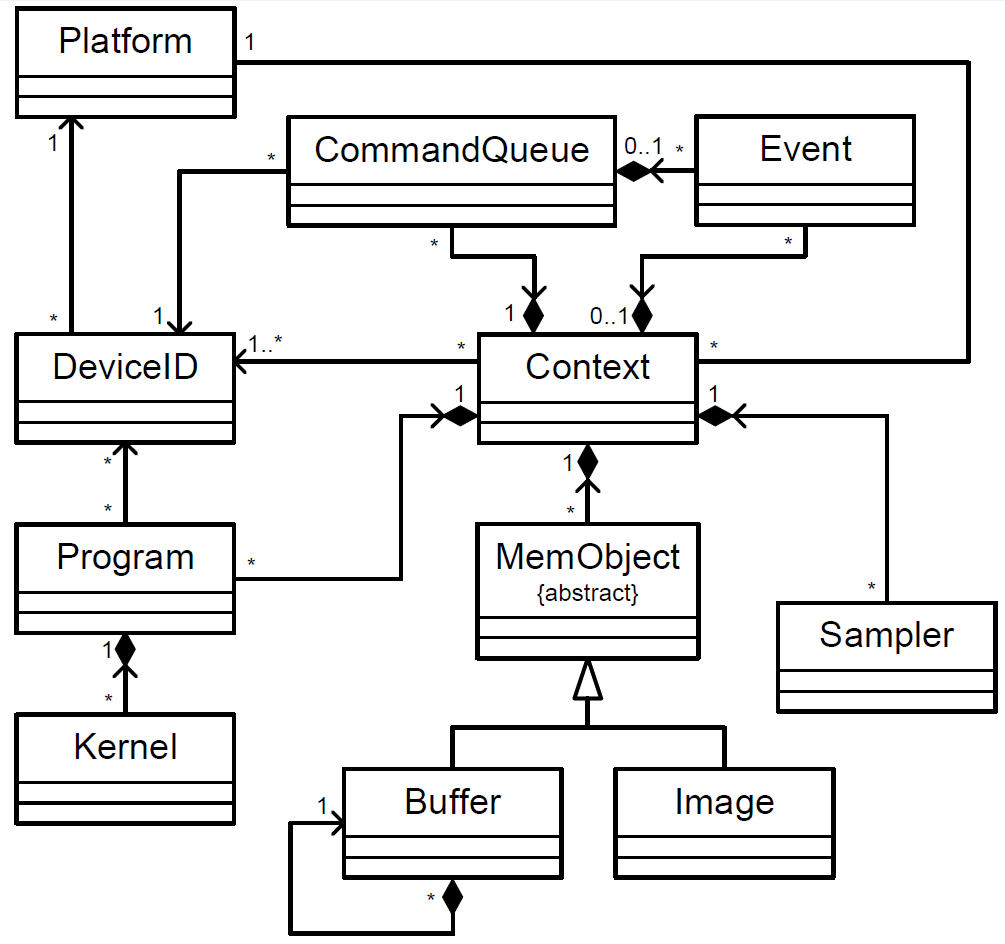
\includegraphics[width=0.6\textwidth]{opencl_uml}
\caption{OpenCL class diagram from the OpenCL 1.2 specification. \cite{opencl_spec}}
\label{fig:opencl_uml}
\end{figure}

\subsection{Platform model}
As OpenCL is an open standard it can be adopted by any hardware vendor manufacturing powerful enough processors to support the features specified by the Khronos Group. Many computers contain more than one of such processors; typically at least a CPU and a graphics card, which are both very suitable to be used by OpenCL. However, these devices do not have to share the same OpenCL implementation. On the one hand, someone may have an NVIDIA graphics card using NVIDIA's driver and, on the other hand, have an Intel Core using their OpenCL CPU driver. And then, if somebody has an AMD Radeon graphics card with AMD's Catalysts driver, the CPU can also be accessed using the same driver.
This situation of multiple available OpenCL implementations on the same machine is handled by the platform model. Each OpenCL implementation on the system (a vendor specific driver) represents a platform. The available platforms on the system, which in this context is often called the host, can be queried using the \lstinline!clGetPlatformIDs! function (for a source code sample see chapter \ref{sec:code_sample}).
Each platform supports one or more devices (the hardware supported by the driver). Reconsidering the previous scenario, the Intel platform would support one device, which is the CPU, whereas the AMD platform would support both the GPU and the CPU. The available devices of a platform can be retrieved by calling \lstinline!clGetDeviceIDs! with the desired platform. Devices available on the same platform (e.g. CPU and AMD GPU using the AMD platform) can be used together which is referred to as heterogeneous computing. 
A device itself consists of multiple compute units being functionally independent from each other (cf. the SMs of a GPU). Each compute unit itself is then eventually subdivided into processing elements (cf. the cores inside a SM). The number of available compute units on a device and much other information like memory capacities can be queried using \lstinline!clGetDeviceInfo!.
Figure \ref{fig:platform_model} visualizes the relation of platforms, devices, compute units and processing elements. \cite[p.19ff]{opencl_book}

\begin{figure} 
\centering
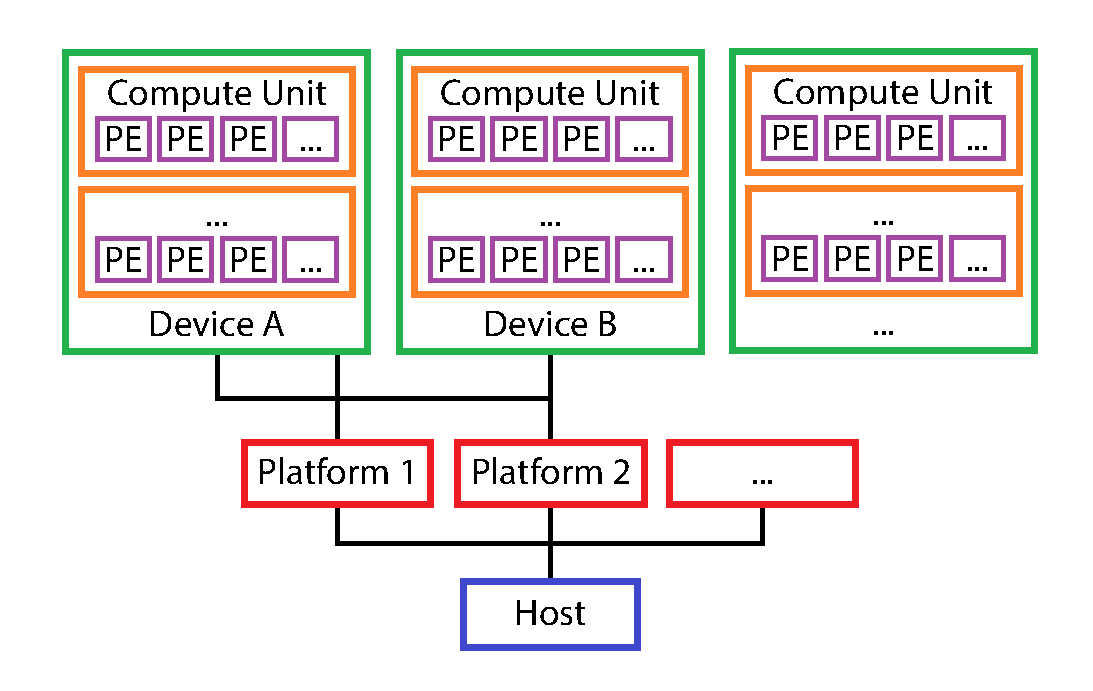
\includegraphics[width=0.7\textwidth]{platform_model}
\caption{OpenCL's platform model.}
\label{fig:platform_model}
\end{figure}

\subsection{Execution model}
\label{sec:execution_model}
The central component of OpenCL's execution model are kernels. But before a kernel can be executed on a device, a number of additional resources have to be set up.
After a device has been selected, a context has to be created that manages objects like memory buffers or kernels associated with the device. A context is created by calling \lstinline!clCreateContext! with one or more devices of the same platform as arguments. Additionally, properties may be passed to the function, like a platform to restrict the context to this platform allowing multiple contexts to different platforms to coexist, or a handle to an OpenGL (Open Graphics Library, a 3D API) context to enable graphics interoperability. \cite[p.22]{opencl_book}

While a context holds static objects shared between the host and one or more devices, OpenCL offers an additional mechanism for host device communication. To request action from a device, a command queue needs to be created within a context and associated with this device. This is done by calling \lstinline!clCreateCommandQueue! with the context and device as arguments. Once a command queue is created, the host can request actions from the device by enqueuing operations like memory buffer writes/reads or kernel executions. Per default these operations are executed asynchronously to the host application, although explicit synchronization can be enforced by calling \lstinline!clFinish! on the command queue, which blocks until all pending operations have been completed. \cite[p.22, 23, 26]{opencl_book}

\subsubsection{Creating kernels}
After the OpenCL execution environment has been successfully prepared, all that is left is the actual piece of code to execute. OpenCL C code is usually written into text files just as every other code. But in contrast to the host application, OpenCL C code is not compiled before an OpenCL application is deployed. OpenCL C code is compiled at runtime via corresponding API functions. This peculiarity is required as different vendors use individual binary codes that may be executed on their devices.
Therefore, an application has to read the OpenCL C code from the shipped source files at runtime and pass it to the \lstinline!clCreateProgramWithSource! function which returns a program object representing the given piece of code. This program can be compiled and linked for one or more devices by calling \lstinline!clBuildProgram!. As compile errors can occur (return value is not equal to \lstinline!CL_SUCCESS!) the compile log may be retrieved by a subsequent call to \lstinline!clGetProgramInfo!. After the program has been successfully built, kernels can be extracted (a program may contain multiple kernels). This is done by calling \lstinline!clCreateKernel! with the compiled program and the name of a function with the \lstinline!__kernel! attribute, which will be used as entry point into the kernel. The obtained kernel is ready for being enqueued on a command queue to a device the kernel was compiled for. \cite[p.26, 27]{opencl_book}

\subsubsection{Kernel execution}
\label{sec:kernel_execcution}
A kernel can be seen as C function that is executed in parallel on the device's processing resources by the OpenCL runtime. As elaborated in chapter \ref{sec:hardware_arch}, these resources may be organized very differently. Therefore OpenCL uses an abstraction model describing the dimensions of the queued work and how it is split up into small pieces. \cite[p.16]{opencl_book}

When the host application wants to enqueue a kernel, it has to specify the size of the problem as a so-called n-dimensional range (NDRange). This range can be seen as a one-, two- or three-dimensional grid of indexes which typically represent the size of the input or output of a kernel. Each element of the grid represents a single kernel invocation and is called a work item. Work items are identified by their position inside the grid which is named global id. The size of the grid is called the global work size. \cite[p.18]{opencl_book}

For example: a matrix multiplication with an output matrix of $M*N$ elements might enqueue a kernel with a two-dimensional range of $M*N$ work items. Each work item would then use it's indexes to determine the row and column of the input matrices and the position of the calculated output value.

To closer adapt to GPU hardware architectures, the NDRange can be equally divided into work groups. Work items inside a work group benefit from having a dedicated shared memory block available. Access to this memory can be synchronized between the work items of a work group providing a basic method of communication. To address a work item inside a work group, each work item has an additional local id and a group id. The extends of a work group must be of the same dimension as the NDRange and the sizes in each dimension, called local work sizes, must be powers of two and evenly divide the global work sizes. \cite[p.18]{opencl_book} The maximum number of work items in a work group is implementation dependent and can be queried by a call to \lstinline!clGetDeviceInfo! with the \lstinline!CL_DEVICE_MAX_WORK_GROUP_SIZE! constant as argument. Figure \ref{fig:NDRange} shows the relation of the NDRange, work groups and work items. 

\begin{figure} 
\centering
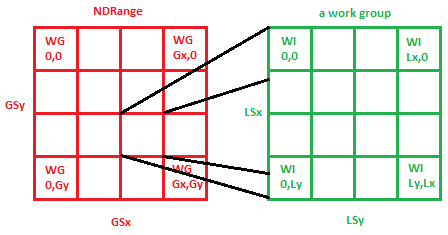
\includegraphics[width=0.6\linewidth]{NDRange}
\caption{The two-dimensional NDRange consisting of $GSx * GSy$ work groups. Each work group consists of $LSx * LSy$ work items. A work item has two indexes in each dimension, the local index (relative to the work group) and a global index (relative to the NDRange), as well as the indexes of the group it is part of. The local work sizes are LSx and LSy whereas the global work sizes are $GSx * LSx$ and $GSy * LSy$.}
\label{fig:NDRange}
\end{figure}

A kernel is executed on a command queue by calling \lstinline!clEnqueueNDRangeKernel!. Additional important arguments beside the kernel and the command queue are the NDRange's dimensions, the global work size and the local work size. The local work size is optional. Before a kernel is executed, arguments may be specified for the \lstinline!__kernel! function according to the function's signature. These arguments are passed to the device when the kernel starts executing and can be accessed via the \lstinline!__kernel! function's parameters. Arguments are set from the host by calling \lstinline!clSetKernelArg! with the argument's index in the kernel function's signature as well as the size and value of the argument.

\subsubsection{Kernel code}
The language kernels are written in is OpenCL C, which is derived from C99 and extended by OpenCL specifics like vector data types, built in functions and additional key words. A kernel function must have the \lstinline!__kernel! attribute and must have void as it's return type. The function's name identifies the kernel to the host. A kernel may have parameters which are declared in the function's signature. An example kernel function for a matrix multiplication is given in listing \ref{lst:kernel_example}.

\lstset{basicstyle=\ttfamily{}\scriptsize{}}
\begin{lstlisting}[caption={An example of a kernel function's signature.},label={lst:kernel_example},language=CL]
__kernel void matrixMultiplication(int n, int m, __global const float* matrixA,
		__global const float* matrixB, __global float* output) {
	// kernel code ...
}
\end{lstlisting}
\lstset{basicstyle=\ttfamily{}}

\subsection{Memory}
Many applications often have to work with large amounts of data. As the data that can be passed to a kernel function by value is restricted to a small size, OpenCL offers the possibility to allocate larger blocks of memory represented as a memory object which is valid inside a context and moved to a device when necessary. At the very top OpenCL defines two basic types of memory, buffers and images. Buffers can be seen as a continuous block of memory equivalent to an array in C allocated using \lstinline!malloc!. Images in contrast are abstract memory objects which can make use of device specific hardware acceleration and optimization when being read from or written to (e.g. texture units on a GPU). Images do not have to be supported by a device. \cite[p.23f]{opencl_book}

\subsubsection{Buffers}
Buffers are created by the host application via a call to \lstinline!clCreateBuffer!. In addition to the context and buffer size, several flags may be specified. With these flags (beside further options) the buffer can be declared as read or write only, or OpenCL can be instructed to use or copy a provided block of host memory. Once a buffer is created, read and write operations may be enqueued on a command queue to transfer a buffer's content (or parts of it) between the host and a device. \lstinline!clEnqueueReadBuffer! and \lstinline!clEnqueueReadBuffer! are the corresponding API functions for transferring memory. When needed by a kernel, buffers have to be set as arguments to a kernel and can be accessed via a pointer from inside the kernel function. \cite[p.24]{opencl_book}

\subsubsection{Images}
\label{sec:images}
Images abstract the underlying storage implementation to allow a device to use hardware optimizations. GPUs for example might use their texture units for improved read and write access as well as providing hardware accelerated interpolation between pixel values of the image. As images do not need to be represented as continuous arrays of a specified data type, a format descriptor is used to determine the size and data type of a pixel value of the image. Images are created by a call to \lstinline!clCreateImage2D! or \lstinline!clCreateImage3D! (unified to \lstinline!clCreateImage! in OpenCL 1.2) with similar parameters as the buffer creating functions. Additionally, the image format descriptor has to be specified and an optional padding between the rows of the image can be set. Images are read and written by the host application via calls to \lstinline!clEnqueueReadImage! and \lstinline!clEnqueueWriteImage!. Like buffers, images can be set as arguments to a kernel, but cannot be accessed via pointers inside the kernel function. Special built-in functions like \lstinline!read_imagef! have to be used in combination with a sampler object which determines out-of-bounds image access, interpolation, and access coordinate handling. \cite[p.25f]{opencl_book}

\subsubsection{Memory model}
As memory subsystems are highly diverse between different kinds of hardware devices, OpenCL defines an abstract memory model giving vendors the possibility to map OpenCL's abstract types of memory to physical memory units on a device.
OpenCL defines four different types of memory which are shown in figure \ref{fig:memory_model}:

\begin{figure} 
\centering
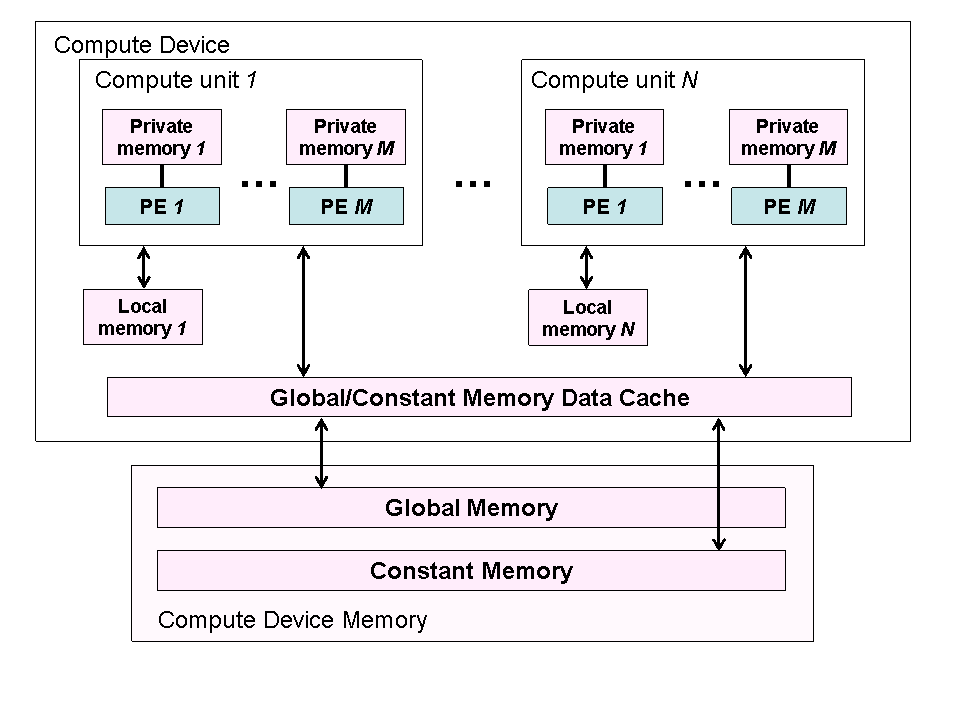
\includegraphics[width=0.6\linewidth]{memory_model}
\caption{Memory model as defined by the OpenCL 1.2 specification.\cite{opencl_spec}}
\label{fig:memory_model}
\end{figure}

\begin{description}
	\item[Global memory] \hfill \\
	Global memory is the largest of all memory regions and visible to all compute units on a device. This memory region is used whenever data is copied to or from a device. Buffers and images are allocated in this memory. All pointer variables pointing into global memory have to be prefixed with the \lstinline!__global! attribute inside a kernel. \cite[p.29]{opencl_book}
	
	\item[Constant memory] \hfill \\
	Constant memory is typically implemented as part of the global memory and is used to store read only data which is needed by all work items. All pointer variables pointing into constant memory have to be prefixed with the \lstinline!__constant! attribute inside a kernel. \cite[p.30]{opencl_book} Newer types of hardware may provide special caches for this kind of memory (cf. the read-only data cache in NVIDIA's Kepler architecture in figure \ref{fig:kepler_arch}).
	
	\item[Local memory] \hfill \\
	Local memory (or shared memory) is a small block of memory which is shared between all work items inside a work group. As access to local memory is very fast it can be seen as a programmer controlled cache to global memory. Local memory is often used for preloading data needed by all work items of a work group or to synchronize work items across a work group. All pointer variables pointing into local memory have to be prefixed with the \lstinline!__local! attribute inside a kernel. Local memory can be allocated statically inside a kernel by declaring a fixed sized array like \lstinline!__local float sharedArray[32];! or dynamically with a call to \lstinline!clSetKernelArg! providing the size of the local memory block requested and \lstinline!nullptr! as pointer to the arguments value. \cite[p.30]{opencl_book}

	\item[Private memory] \hfill \\
	Private memory belongs to each work item itself and is typically stored in registers (on a GPU) except a work group requests more memory than the available register file. In this case the spilled private memory is mapped to global memory. Private memory cannot be allocated, but pointers to local variables may be used to pass values by reference to functions called by the kernel function. Pointers to variables pointing to private memory can be prefixed with the \lstinline!__private! attribute inside kernels, but they do not have to as \lstinline!__private! is the default pointer type. \cite[p.30]{opencl_book}
\end{description}

\subsection{Code sample}
\label{sec:code_sample}

The following piece of code in listing \ref{lst:opencl_example} shows a minimal OpenCL application with a kernel that calculates the sum of two input vectors. To keep the code simple no error handling is performed, only the error code is retrieved. The codes in the subsequent implementation chapters will completely go without error handling or error code retrieval.

\pagebreak

\lstset{basicstyle=\ttfamily{}\scriptsize{}}
\lstinputlisting[language=C++,caption=A minimalistic working OpenCL application which calculates the sum vector of two large input vectors.,label=lst:opencl_example]{code/sample/main.cpp}
\lstset{basicstyle=\ttfamily{}}

The first step in every OpenCL program is to choose a platform. As platforms correspond to the available OpenCL implementations on the system, multiple platforms can be available. The example code only queries the first available OpenCL platform by calling \lstinline!clGetPlatformIDs! with 1 and a pointer to a variable able to hold one platform id as arguments. The third parameter could be used to retrieve the number of actually available platforms. \\
After a platform has been chosen, we can continue by choosing a device for this platform which works analogously as selecting a platform. In addition to specifying the platform to query devices for, OpenCL also allows us to define the type(s) of devices we would like to get. In this case we would like to have the first available GPU on the first available platform by specifying \lstinline!CL_DEVICE_TYPE_GPU! when calling \lstinline!clGetDeviceIDs!\footnote{Calling \lstinline!clGetDeviceIDs! with a device type as argument may return no devices. The Intel OpenCL platform for example only supports CPUs and therefore does not provide a GPU device. Appropriate error handling is necessary in real world applications.}. To be able to allocate OpenCL resources and enqueue operations on a device we now have to create a context and a command queue using \lstinline!clCreateContext! and \lstinline!clCreateCommandQueue!. Further arguments to both API functions allow specifying further properties which can be looked up in the corresponding documentation. \\
The program is now ready to create a kernel. OpenCL kernel source code is typically placed in a file and read at runtime. For simplicity, the kernel code of this example is emplaced into the host code as string literal. The OpenCL kernel simply queries the id of the current work item, loads the values from the buffers \lstinline!a! and \lstinline!b! at this index and writes the sum of them to buffer \lstinline!c! at the same index. \\
To create an actual kernel object within the context, we first have to create an OpenCL program out of the source code which is done by calling \lstinline!clCreateProgramWithSource! and passing the source code as argument. Furthermore, the program has to be compiled for the chosen device. By calling \lstinline!clBuildProgram! the source code of the program object is compiled and linked into an executable for the specified device. This step can take up to several seconds. Similar as building programs in other languages, the compiling may fail. In this case an error code is returned and a compiler log could be retrieved using \lstinline!clGetProgramBuildInfo!.
On a successful build, the kernel object (which can be seen as entry point into the program) can be finally retrieved by calling \lstinline!clCreateKernel! and specifying the compiled program as well as the name of the \lstinline!__kernel! function. \\
Before we can execute the kernel we have to allocate storage for the input and output data. Three arrays are allocated on the host with a size of \lstinline!N!. The first two are filled with data. To move the data to the GPU, three buffer objects have to be created using \lstinline!clCreateBuffer! having the same size as the corresponding host arrays. Note that the two input buffers are created as read only and the output buffer as write only by setting appropriate flags. To initiate the copy operations from the host to the GPU device, buffer write operations have to be enqueued on the command queue using \lstinline!clEnqueueWriteBuffer!. Arguments are the command queue, the buffer to write to, a boolean specifying if the write operation should be blocking, the offset and length of the region to be written to, a pointer to the host memory from which should be read and several further arguments concerning events which will not be covered. By specifying \lstinline!false! for the blocking write parameter, the write operation is execute asynchronously to the host program. Therefore the provided host pointers (\lstinline!a! and \lstinline!b!) have to be available at least until the first blocking OpenCL call. Asynchronous memory transfers are advantages, as OpenCL may decide itself when to perform the actual copy. Furthermore, multiple copies may be executed concurrently and even beside kernel executions.\\
Now it is time to setup and execute the kernel. The three buffer objects, on which the kernel will operate, are set as the kernel's arguments via \lstinline!clSetKernelArg!. The second parameter specifies the index of the argument in the order they appear in the kernel function's signature. Finally, the kernel can be enqueued to be executed using \lstinline!clEnqueueuNDRangeKernel!. The problem is one-dimensional with a global work size of \lstinline!N!. The local work size is not specified and therefore determined by OpenCL. Similar to the buffer writes, the kernel enqueue operation is also executed asynchronously. However, the arguments do not have to be available anymore after \lstinline!clSetKernelArg! returns as they are copied by the OpenCL implementation. Furthermore, as the kernel depends on the buffer objects as inputs, the kernel is not executed until all buffer operations (memory transfers) on the inputs have completed. \\
The last step is to read the results back to host memory via \lstinline!clEnqueueReadBuffer! having the same arguments as the corresponding write function. This time however, the synchronization boolean is set to \lstinline!true!. Therefore, the function call blocks until the read operation has finished. Afterwards the result on the host may be further processed (e.g. printed). \\
When OpenCL resources are no longer needed, they should be released using their corresponding \lstinline!clRelease*! API functions.